\documentclass[12pt,a4paper]{report}
\linespread{1.2}

\usepackage{amsmath,amssymb,amsfonts}
\usepackage{algorithmic}
\usepackage{graphicx}
\usepackage{xcolor}
\usepackage{multirow}
\usepackage{float}
\usepackage{listings}
\usepackage{listings-golang}
\lstset{ % add your own preferences
    frame=single,
    basicstyle=\linespread{0.9}\footnotesize\ttfamily,
    keywordstyle=\color{red},
    numbers=left,
    numbersep=5pt,
    showstringspaces=false, 
    stringstyle=\color{blue},
    tabsize=4,
    language=Golang % this is it !
}
\lstdefinelanguage{yaml}{
  keywords={true,false,null,y,n},
  keywordstyle=\color{darkgray}\bfseries,
  ndkeywords={},
  ndkeywordstyle=\color{black}\bfseries,
  identifierstyle=\color{black},
  sensitive=false,
  %moredelim=[l]{}{:},
  comment=[l]{#},
  morecomment=[s]{/*}{*/},
  commentstyle=\color{purple}\ttfamily,
  stringstyle=\color{blue}\ttfamily,
  %morestring=[l]{-}{},
  morestring=[b]',
  morestring=[b]"
}
\usepackage[font={small,it}]{caption}
\usepackage[english,ngerman]{babel}
\usepackage[backend=biber,
            sorting=none,   % Keine Sortierung
            doi=true,       % DOI anzeigen
            isbn=true,      % ISBN nicht anzeigen
            url=true,       % URLs anzeigen
            maxnames=6,     % Ab 6 Autoren et al. verwenden
            minnames=1,     % und nur den ersten Autor angeben
            style=numeric-comp,]{biblatex}
\addbibresource{literatur.bib}
\usepackage[colorlinks=true,
            urlcolor=black,
            linkcolor=black,
            filecolor=black,
            citecolor=black,]{hyperref}

\def\BibTeX{{\rm B\kern-.05em{\sc i\kern-.025em b}\kern-.08em
    T\kern-.1667em\lower.7ex\hbox{E}\kern-.125emX}}

\begin{document}

\title{Erzeugung, Aufzeichnung und Wiedergabe von Netzwerk-Unterbrechungen in einer Testumgebung für verteilte Systeme}


\author{Jonathan Arns
	\textit{Hochschule Mannheim} \\
	Fakultät für Informatik\\
	Paul-Wittsack-Str. 10\\
	68163 Mannheim\\
	jonathan.arns@stud.hs-mannheim.de
}

\maketitle

\tableofcontents
\setlength{\parindent}{0em}
\setlength{\parskip}{0.5em}

%%%%%%%%%%%%%%%%%%%%%%%%%%%%%%%%% Document beginning %%%%%%%%%%%%%%%%%%%%%%%%%%%%%%%%%%%%%%

\begin{abstract}
	Das ist das abstract, das werde ich wohl am Ende schreiben.
\end{abstract}


\chapter{Einleitung}
\cite{analysis_of_network_partition_failures}
\cite{chaos_engineering}
\chapter{Grundlagen}
\section{Verteilte Systeme}
\subsection{Partition Tolerance}
\subsection{CAP}
\subsection{Linearisierbarkeit}
\subsection{Verteilter Consens}
\section{Docker}
Docker als leichtgewichtige Alternative zu virtuellen Maschinen ist inzwischen weitgehen bekannt und bildet das Rückrad vieler
moderner Cloud Anwendungen. Verteilte Microservice-basierte Systeme laufen heute fast ausschließlich in Containern und damit oft
in Docker oder ähnlichen Technologien.
\section{Proxy}

\chapter{State of the Art}
\cite{debugging_distributed_systems_2016}
\section{Tracing}
\section{Failure / Chaos Testing}
Failure Testing ist eine Familie von Ansätzen zum Testen der Fehlertoleranz verteilter Systeme. Die Grundidee ist immer, als
Client mit dem System zu interagieren und zeitgleich die Umgebung des Systems zu manipulieren, beispielsweise mit
Netzwerk-Unterbrechungen. Failure Tests werden als automatisierte Integrationstests über eine Programmierschnittstelle definiert
und beinhalten den Auf- und Abbau des Systems, eine Reihe definierter Interaktionen mit dem System und in der Regel zufällige
Fehler-Injektionen in die Systemumgebung. Zusätzlich wird oft nach Tests die Einhaltung von Invarianten des Systems anhand eines
Modells geprüft, um in zufallsgetriebenen Tests automatisch Bugs identifizieren zu können.

\cite{why_is_random_testing_effective}
\cite{failify_masters_thesis}
\subsection{Jepsen}
Jepsen ist ein Failure-Testing-Framework in der Sprache Clojure, welches speziell auf das Verhalten von verteilten Systemen bei
Netwerk-Unterbrechungen u.Ä. ausgerichtet ist. Jepsen hat sich auf dem Gebiet zu einem Industriestandart für das Testen von
verteilte Datenbanken entwickelt \cite{abstracting_the_geniuses} und wird für Projekte wie MongoDB, etcd, VoltDB, Hazelcast,
Elasticsearch und CockroachDB verwendet und hat in jedem dieser Systeme bereits reale Bugs aufgedeckt \cite{jepsen_analyses}.

Bei Jepsen-Tests werden auf einem Kontrollknoten eine Reihe von Client Prozessen ausgeführt, die Requests an das SUT senden.
Gleichzeitig werden mit Hilfe von sog. Nemesis Prozessen verschiedene Fehler in das System eingeführt. Zur Erzeugung von
Netzwerk-Unterbrechungen verwendet Jepsen die Linux Netwerk Tools wie iptables. Neben Netzwerk-Unterbrechungen ist Jepsen in
der Lage, verschiedene andere Fehler zu erzeugen, wie beispielsweise Verzerrungen zwischen den Systemuhren der einzelnen Knoten.
Am Ende eines Tests wird verifiziert, ob alle durchgeführten Operationen unter den Regeln des SUT linearisierbar sind. Sind sie das
nicht, hat Jepsen einen Bug gefunden, vorrausgesetzt die Regeln des SUT sind korrekt modelliert.
\subsection{Replay Debugging}
\cite{distributed_replay_debugging_1997}
% idea exists, seems very promising
% different approaches with different advantages and drawbacks
\subsection{Debugger für Verteilte Systeme}
\cite{oddity_graphical_debugger}
\cite{gotcha_interactive_debugger}

\section{Was fehlt noch?}
% hier kommt future work of existing papers

% leicht verwendbare chaos failure testing
% zuverlässige reproduktion von bugs

\chapter{Systembeschreibung}
Dieses Kapitel beschreibt die Idee, die Anforderungen und die Umsetzung des im Rahmen dieser Arbeit entwickelten Systems ditm.
\section{Idee}
Die grundlegende Idee dieser Arbeit ist ein Tool, welches die Ideen des Failure Testings mit denen des Record and Replay
Debuggings vereint. Dieses Tool soll nach Record and Replay Prinzip beim Debugging von Bugs im Zusammenhang mit
Netwerk-Unterbrechungen in verteilten Systemen helfen. Mit Hilfe des Tools sollen wie beim Failure Testing Netwerk-Unterbrechungen
während Test Durchläufen simuliert werden, allerdings nicht wie beim Failure-Testing in programmatisch von vorn herein definierten
Testfällen, sondern interaktiv, während der Nutzer mit dem System interagiert. Um gefundene Bugs dennoch zuverlässig reproduzieren
zu können, soll das Tool Situationen aufzeichnen und zum späteren Zeitpunkt wieder abspielen können, insbesondere mit den gleichen
simulierten Netzwerk-Bedingungen wie während der Aufzeichnung.

Ein großer Fokus der Arbeit ist dabei speziell auf dem verfolgten Ansatz für ein solches System. Dieser ist, alle Nachrichten
innerhalb eines verteilten Systems über einen Proxy zu leiten, der diese inklusive Metadaten aufzeichnet und in der Lage ist,
kontrolliert Netwerk-Unterbrechungen zu simulieren, indem einzelne Nachrichten geblockt, bzw. nicht weiter geleitet, werden.  Mit
diesem Aufbau soll auch ein Replay der Netzwerk-Bedingungen anhand eines zuvor durch den Proxy aufgezeichneten Test Durchlaufs
möglich sein, sofern der Proxy in der Lage ist, während des Replays für jeden erhaltenen Request zu identifizieren, welchem
Request aus der Aufzeichnung er jeweils zuzuordnen ist. Zudem muss der Proxy Requests, die in der Aufzeichnung von außerhalb des
Systems kamen, identifizieren und während des Replays zum richtigen Zeitpunkt selbstständig in das System senden.

Ein Proxy wird den anderen, verbreiteteren Fehler-Mechanismen des Failure-Testings vorgezogen, da die Erwartung ist, dass dieser
sich insbesondere besser für Replays eignet. Das liegt daran, dass ein Proxy jede Nachricht des SUT einzeln betrachten und
gegebenenfalls blocken kann, andere Mechanismen, die sich rein auf zeitliche Abstände und die Reihenfolge von Operationen
verlassen, ermöglichen dies nicht ohne weiteres. Dadurch soll das Tool besser mit Unterschieden in der zeitlichen Reihenfolge von
Nachrichten umgehen können, die im Replay auftreten können, zum Beispiel weil Replays schneller als das originale Recording
ablaufen, falls im Recording ein Mensch mit dem SUT interagiert hat, dessen Aktionen deutlich schneller als in Echtzeit agbespielt
werden.

\section{Anforderungen}
ditm ist ein Prototyp, der primär dem Zweck dient, die zuvor beschriebene Idee zu verfizieren.
Die Anforderung reflektieren diesem Umstand, indem beispielsweise die unterstützten Netwerk-Protokolle auf HTTP beschränkt sind.
\subsection{Funktionale Anforderungen}
\begin{table}[H]
	\centering
	\caption{Funktionale Anforderungen}
	\label{tab:fa}
	\begin{tabular}{|l|l|p{7cm}|}
		\hline
		ID   & Anforderung                   & Beschreibung                                                                                                                                                                                                          \\ \hline
		FA1  & Netzwerk Unterbrechungen      & Das System soll kontrolliert Netzwerk-Unterbrechungen zwischen Knoten des zu testenden Systems erzeugen können.                                                                                                       \\ \hline
		FA2  & Aufzeichnung                  & Das System soll den gesamten Netzwerkverkehr des zu testenden Systems aufzeichnen können. Insbesondere sollen auch erzeugte Netzwerk-Unterbrechungen aufgezeichnet werden.                                            \\ \hline
		FA3  & Replay                        & Das System soll anhand einer durch das System erstellten Aufzeichnung die Situation in der Aufzeichnung am laufenden Testsystem wiederherstellen und vor allem inklusive Netzwerk-Unterbrechungen wiedergeben können. \\ \hline
		FA4  & Zufällige Unterbrechungen     & Das System soll Netwerk-Unterbrechungen zufällig erzeugen können.                                                                                                                                                     \\ \hline
		FA5  & Kontrollierte Unterbrechungen & Das System soll dem Nutzer die Möglichkeit geben, Netwerk-Unterbrechungen konkret zu steuern.                                                                                                                         \\ \hline
		FA6  & Log Aggregation               & Das System soll zusätzlich zum Netzwerkverkehr auch die Log ausgaben des zu testenden Systems aufzeichnen und aggregieren können.                                                                                     \\ \hline
		FA7  & Log Matching                  & Das System soll die aufgezeichneten Nachrichten und Logs in chronologischer Reihenfolge gemeinsam anzeigen können.                                                                                                    \\ \hline
		FA8  & Volume Snapshots              & Das System soll für zustandsbehaftete Systeme Snapshots der Docker Volumes erstellen und zu einem späteren Zeitpunk wiederherstellen können.                                                                          \\ \hline
		FA9  & Nachrichten von außen         & Das System soll dem Nutzer Schnittstelle bieten, über die Nachrichten reproduzierbar von außen in das zu testende System gesendet werden können, um Prozesse im zu testenden System anzustoßen.                       \\ \hline
		FA10 & Responses Blocken             & Das System soll in der Lage sein, nicht nur Requests auf dem Hinweg zum Server zu blockieren, sondern optional auch erst die Antwort auf dem Rückweg.                                                                 \\ \hline
	\end{tabular}
\end{table}

\subsection{Nicht-Funktionale Anforderungen}
\begin{table}[H]
	\centering
	\caption{Nicht-Funktionale Anforderungen}
	\label{tab:nfa}
	\begin{tabular}{|l|l|p{7cm}|}
		\hline
		ID   & Anforderung              & Beschreibung                                                                                                                                                                                                  \\ \hline
		NFA1 & Portabilität             & Das System soll vollständig in Docker lauffähig sein und mittlels docker-compose konfigurierbar sein.                                                                                                         \\ \hline
		NFA2 & Proxy Architektur        & Umsetzung des Konzepts, einen Proxy zur erzeugung etc von Partitionen zu verwenden                                                                                                                            \\ \hline
		NFA3 & HTTP                     & Das System soll mit HTTP als Netzwerkprotokoll Arbeiten und grundlegend alle verteilten Systeme, die ausschließlich über HTTP kommunizieren und die Umgebungsvariable HTTP\_PROXY respektieren, unterstützen. \\ \hline
		NFA4 & Deterministische Replays & In der Wiedergabe einer Aufzeichnung sollen immer genau die Teile des Netzwerkverkehrs geblockt werden, die auch in der Aufzeichnung vom System geblockt wurden. Nicht mehr, nicht weniger und keine anderen. \\ \hline
		NFA5 & Usability                & Das System soll einfach über eine graphische Oberfläche bedienbar sein.                                                                                                                                       \\ \hline
		NFA6 & Echtzeit                 & Requests und Logs einer laufenden Aufzeichnung sollen in Echtzeicht angezeigt werden.                                                                                                                         \\ \hline
		NFA7 & Default Test System      & Das zu testenden System sollte für den Test nicht angepasst werden müssen.                                                                                                                                    \\ \hline
	\end{tabular}
\end{table}

\section{Architektur}
Das Herzstück des Systems ist entsprechend der Idee ein eigens entwickelter HTTP Proxy, welcher den Netzwerk-Verkehr in einem
verteilten System aufzeichnen und Nachrichten wahlweise nicht weiter leiten kann. Dieser Proxy läuft in einem Docker Container
direkt neben dem SUT und ist auch Teil des gleichen Docker Netzwerks wie das SUT. Außer dem Proxy hat ditm eine weitere eigens
entwickelte Komponente, ein Docker-Log-Driver-Plugin, welches Container-Logs an den Proxy sendet. Die Datenflüsse zwischen
Komponenten des Systems sind in Abbildung \ref{fig:dataflow} im Kontext eines SUT mit zwei Knoten dargestellt.
\begin{figure}[H]
	\centering
	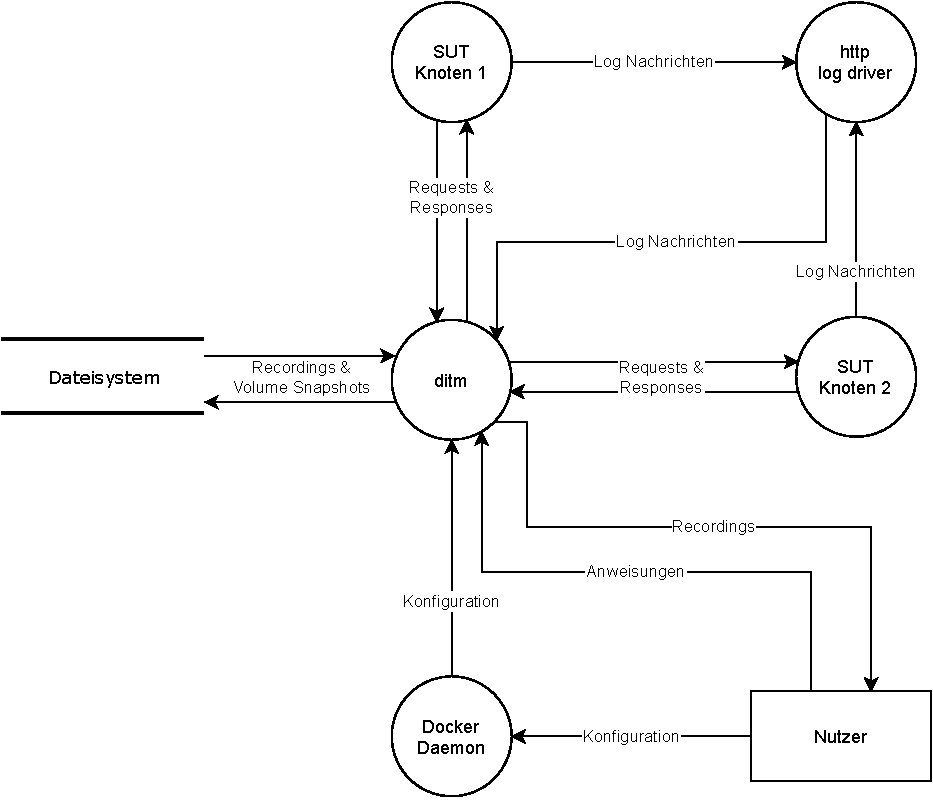
\includegraphics[width=\linewidth]{img/ditm-Dataflow.pdf}
	\caption{Datenflussdiagramm für ditm}
	\label{fig:dataflow}
\end{figure}

\subsection{Datenmodell}
Das Datenmodell von ditm ist einfach gehalten. Das Top Level Datenobjekt ist das Recording, dieses enthält zwei chronologisch
geordnete Listen, eine mit den Log Nachrichten des SUT und eine mit den aufgezeichneten Requests. Beide Listen enthalten
die jeweiligen Objekte für alle Knoten des SUT, ohne diese weiter voneinander zu trennen. Sollte eine gefilterte Liste
benötigt werden, die nur Objekte für bestimmte Knoten enthält, wird diese dynamisch erzeugt. Recordings enthalten außerdem
eine Referenz auf einen Volume Snapshot, sofern für das Recording einer existiert.
Die eigentlichen Request Datenobjekte enthalten neben dem Request Body eine Menge Metadaten, die teilweise vom Request selbst
stammen und teilweise durch ditm erzeugt wurden, beispielsweise ob der Request geblockt wurde oder nicht.
Log Nachrichten umfassen neben der eigentlichen Nachricht ebenfalls wichtige Metadaten, wie den Namen des Containers, der die
Nachricht geloggt hat. In Abbildung \ref{fig:class} ist das beschriebene Datenmodell in einem Klassendiagramm dargestellt. Die
Implementierungen des Matcher-Interfaces fehlen im Klassendiagramm, da sich hier keine Unterschiede zwischen den einzelnen
Implementierungen zeigen würden und diese gesondert in Kapitel ... behandelt werden. Die Methoden der Klasse Proxy wurden
ebenfalls aus Platzgründen weg gelassen und da diese hier konkret von geringerem Interesse sind. Ein Proxy nimmt im Prototypen die
Rolle eines Gottobjekts ein, dieses Design-Pattern wurde für den Prototypen solideren Patterns vorgezogen, um die Entwicklung
einfach zu halten und Erweiterungen, bzw. Änderungen des Datenmodells währenddessen zu erleichtern.
\begin{figure}[H]
	\centering
	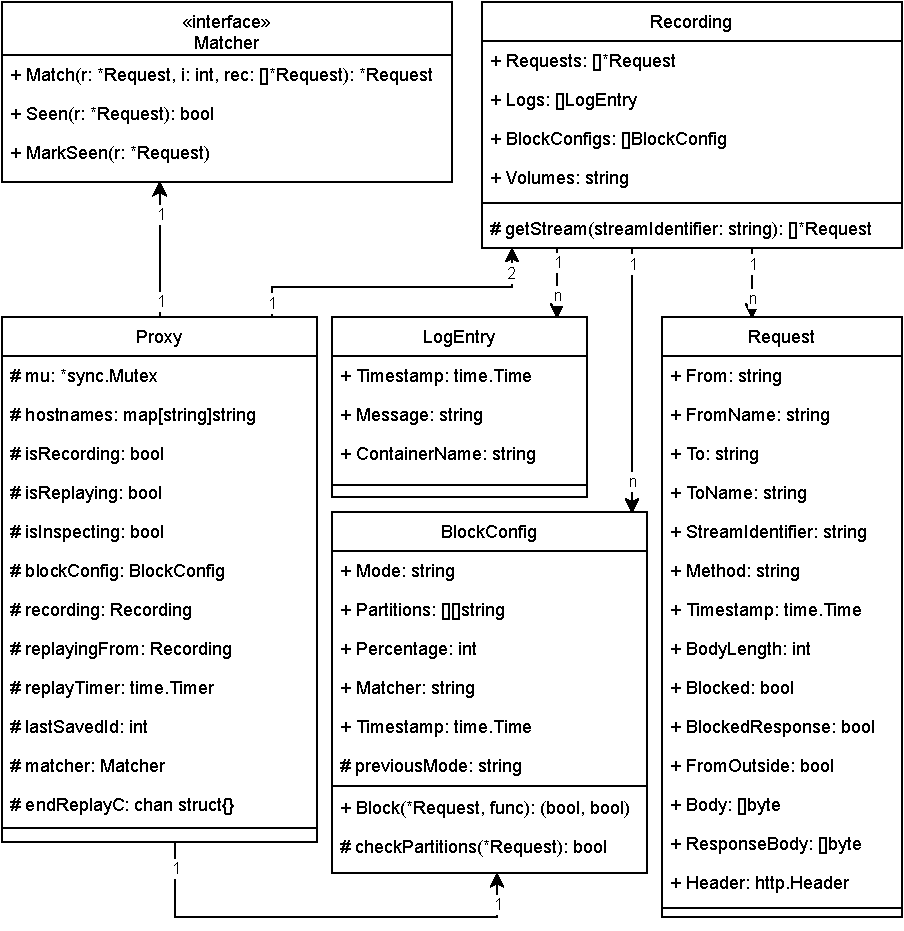
\includegraphics[width=\linewidth]{img/ditm-Class.pdf}
	\caption{Klassendiagramm für ditm ohne Proxy-Methoden und Matcher-Implementierungen}
	\label{fig:class}
\end{figure}

\subsection{Weg eines Requests}
Um eine konkrete Vorstellung von der Arbeitsweise des Proxys zu vermitteln, wird im folgenden beispielhaft der Weg eines
Requests durch das System beschrieben. In diesem Kontext wird der Ursprung des Requests als Client und das Ziel des
Requests als Server bezeichnet, beide sind Knoten des SUT. Abbildung \ref{fig:activity} stellt zunächst den groben Ablauf auf Systemebene dar.
Wichtig ist zu bemerken, dass der Proxy bereits beim ersten erhalten des Requests die komplette Analyse durchführt und
nicht nur entscheidet, ob der Request geblockt werden soll, sondern die Entscheidung auch direkt für die Response trifft,
ohne die Response jemals gesehen zu haben. Tatsächlich wird die Response gar nicht von ditm betrachtet, stattdessen wird
die Analyse vollständig am Request durchgeführt. Die einzige Interaktion des Proxys mit der Response ist, diese zur Anzeige im
Frontend aufzuzeichnen, sie zu blocken falls vorher festgelegt oder sie ansonsten direkt weiter zu leiten.
Der Grund dafür ist, dass fast alle für ditm relevanten Metadaten bereits aus dem Request abgeleitet werden können. Zwar
könnten die Länge der Response und die Response Header möglicherweise ebenfalls von Interesse sein, der Kompromiss wird
hier aber in Kauf genommen, da das die Implementierung erheblich vereinfacht und auch so genügend Metadaten vorliegen,
um verschiedene Algorithmen zur Entscheidung, ob ein Reqeust im Replay geblockt werden soll, zu evaluieren.
Die verschiedenen Ansätze, die diese Arbeit betrachtet, werden in Kapitel ... behandelt.
\begin{figure}[H]
	\centering
	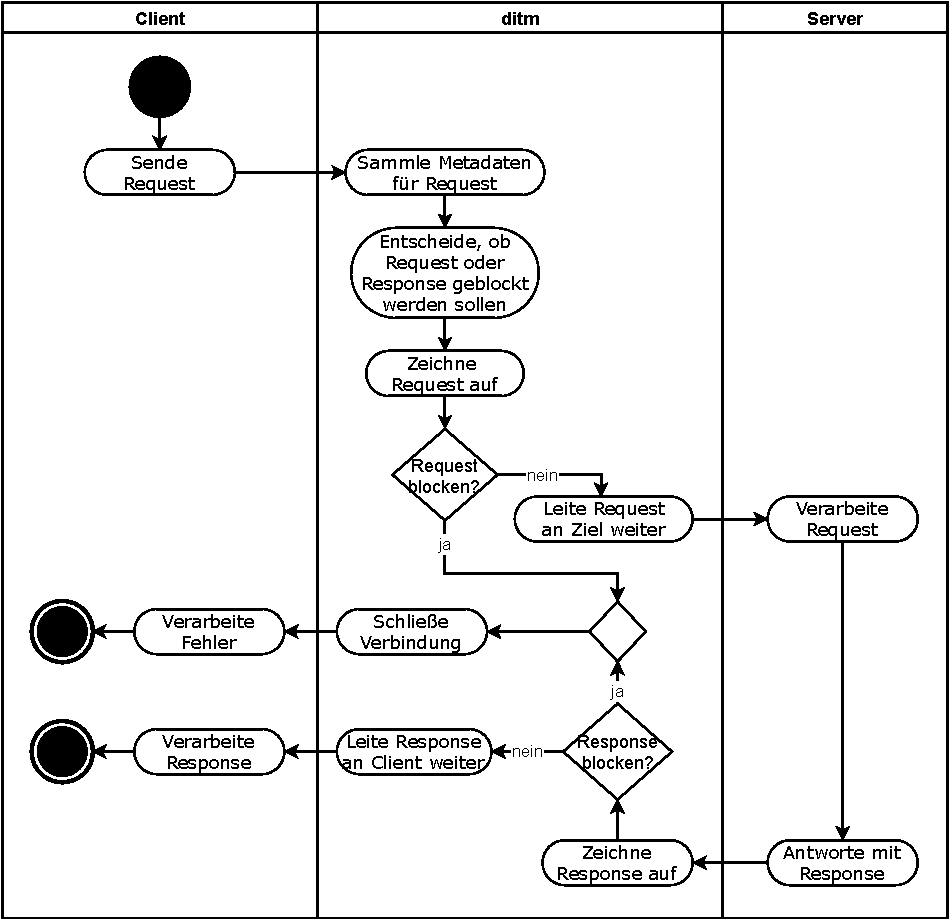
\includegraphics[width=\linewidth]{img/ditm-Activity.pdf}
	\caption{Aktivitätsdiagramm der Interaktion von ditm mit Client und Server eines Requests}
	\label{fig:activity}
\end{figure}

\section{Implementierung}
Als Programmiersprache wird für die Implementierung auf Go gesetzt. Go bietet sich an, da die Standartbibliothek
umfassende, robuste APIs für den Umgang mit Netzwerken bietet und die Sprache insgesamt eine schnelle
Entwicklungsgeschwindigkeit erlaubt, ohne Performance zu vernachlässigen.
\subsection{Datenspeicherung}
Als Speicherformat für ditm wurden einfache Dateien in JSON Format gewählt. So wird jedes Recording Datenobjekt in
einer eigenen Datei serialisiert gespeichert. Dieses Format wurde einer Datenbank aus mehreren Gründen vorgezogen.
Zum einen wird Dateispeicher sowieso für die Volume Snapshots benötigt, die als Zip Dateien gespeichert werden,
es spart also an Komplexität für den Prototypen, für die restlichen Daten ein ähnliches Speichermodel zu wählen.
Zum anderen bieten Dateien den Vorteil, dass der Nutzer die Möglichkeit hat, diese selbst einzeln zu verwalten.
Es ist dem Nutzer also möglich, die Dateien einer einzelnen Aufzeichnung und des zugehörigen Snapshots getrennt
zu sichern oder einfach mit anderen Nutzern über einen generischen Filesharing Dienst zu teilen.
\subsection{Log Driver}
Um die Logging Ausgaben des SUT in ditm aggregieren zu können, muss ditm aus seinem Container heraus auf die Logs der
anderen Container zugreifen. Leider bietet Docker von sich aus keine einfache Möglichkeit dies zu konfigurieren,
stattdessen muss auf Dockers Plugin API zurück gegriffen werden. Immerhin bietet Docker eine spezielle Plugin API
für Log Driver, die es ermöglicht Log Nachrichten durch einen eigenen Driver beliebig weiter zu verarbeiten.
Für ditm wurde ein einfaches Log Driver Plugin entwickelt, welches Nachrichten als HTTP Request an eine beliebige URL
sendet. ditm selbst bietet in seiner API einen Endpunkt an, welcher diese Log Nachrichten empfangen und verarbeiten kann.
\subsection{Frontend}
Als Frontend bietet ditm dem Nutzer eine Web Oberfläche, in der laufende, sowie vergangene, Aufzeichnungen
tabellarisch visualisiert werden können. Des weiteren ist der Proxy vollständig über die GUI kontrollierbar.
Events einer laufenden Aufzeichnung werden in Echtzeicht per Server-Sent-Events Schnittstelle an das Frontend
gesendet und dort dargestellt.
Das Frontend selbst ist eine einfache, serverseitig gerenderte, HTML Seite mit dem notwendigen JavaScript Code,
um SSEs zu empfangen und zu verarbeiten. Die Seite ist mittels Bootstrap gestyled und in Tabs aufgeteilt.
\subsection{Request Matcher}
Die Logik zur Entscheidung, ob ein Request, bzw. eine Response, während eines Replays geblockt werden soll,
ist ein Kernstück des Proxys, welches es ermöglicht, Aufzeichnungen zuverlässig wiederzugeben.
Das Problem lässt sich darauf herunterbrechen, genau den Request im ursprünglichen Recording zu identifizieren,
dem der aktuelle Request während des Replays entspricht. Das liegt daran, dass sich der Proxy während eines
Replays immer exact wie während der Aufnahme verhalten soll.

Der erste Schritt dabei, Requests aus Recording und Replay zu matchen, ist immer die Requests sowohl im
Recording als auch im Replay nach dem StreamIdentifier des aktuellen Requests zu filtern, so dass zwei
kleinere Request Streams entstehen. Der StreamIdentifier wird zusammengesetzt aus den Namen des Clients
und des Servers für den jeweiligen Request, ein so gefilterter Stream stellt also den gesamten Verkehr
zwischen genau zwei Knoten des SUT dar.
Der Rest des Matchings ist wie folgt über ein Interface abstrahiert, um leicht mehrere Implementierungen
austauschen zu können.
\begin{lstlisting}
type Matcher interface {
   	Match(r *Request, i int, rec []*Request) *Request
   	Seen(r *Request) bool
    MarkSeen(r *Request)
}
\end{lstlisting}
Die Methode Match erwartet als Parameter den aktuellen Request, dessen Index im gefilterten Stream des Replays
und den gesamten gefilterten Stream des Recordings und gibt einen Pointer auf den Request im Recording zurück,
der das beste Match darstellt. Die Methoden Seen und MarkSeen dienen dazu, Requests zu markieren, falls sie bereits
im aktuellen Replay vorgekommen sind, bzw. abzufragen, ob ein Request bereits markiert wurde. Es wird also nach jedem Aufruf
von Match der zurück gegebene Request markiert. Eine Methode um Requests zu entmarkieren wird nicht benötigt, da für
jedes Replay ein neuer Matcher initialisiert wird. Insgesamt wurden vier Implementierungen für das Interface mit
verschiedenen Algorithmen für Match erstellt, die im Folgenden dargestellt und später gegeneinander evaluiert werden.
Alle vier Implementierungen verwenden eine Hashtabelle zur Umsetzung der Seen und MarkSeen Funktionalität und ignorieren
bei jedem Aufruf von Match bereits markierte Requests, sowie Requests, die von außerhalt des SUT stammen.
\subsubsection{Zählend}
Mit Abstand der einfachste Request-Matcher ist der zählende Matcher. Dieser bestimmt Matches allein aufgrund der Position
von Requests in den jeweiligen Streams. Es wird also immer der Request als Match bestimmt, welcher im Recording den Index i hat,
wobei i der zweite Parameter der Match Methode ist. Ist der entsprechende Request bereits markiert oder von außerhalb des SUT,
wird kein Match zurück gegeben, was bei allen Matchern dazu führt, dass ditm den Request nicht manipuliert.
Der Zählende Matcher ist nicht als ernsthafter Versuch gemeint, einen guten Matcher zu entwickeln. Vielmehr soll
er als Vergleichsgrundlage für die anderen Matcher dienen.
\subsubsection{Exact}
Alle weiteren Matcher, der Exacte eingeschlossen, verwenden ein Punktesystem, in dem allen Requests des Recordings für verschiedene
Eigenschaften Punkte zugewiesen werden und am Ende der Request mit der höchsten Punktzahl als Match zurück gegeben wird.
Der Exacte Matcher vergibt einen Punkt, falls die Requests an gleicher Stelle in ihren Streams stehen, falls die URIs der
Requests gleich sind, falls die Länge der URIs gleich ist, falls die Bodies gleich sind und falls die Länge der Bodies gleich ist.
Sei i der Index im Replay, j der Index im Recording, req der aktuelle Request im Replay und r der aktuelle
Request im Recording, dann wird der Score für r also wie folgt berechnet.
\begin{lstlisting}
score := 0.0
if i == j {
    score += 1
}
if req.To == r.To {
    score += 1
}
if len(req.To) == len(r.To) {
    score += 1
}
if string(req.Body) == string(r.Body) {
    score += 1
}
if len(req.Body) == len(r.Body) {
    score += 1
}
\end{lstlisting}
Dieser Matcher sollte sich in Situationen mit gemischten Request Reihenfolgen bereits deutlich besser verhalten, als der
einfache zählende Matcher, da er neben der Reihenfolge auch andere Eigenschaften der Requests betrachtet. Trotzdem ist es auch
hier vorstellbar, dass der Matcher deutliche Probleme haben wird, sobald er auf eine Menge ähnlicher Requests trifft, die nur
leicht gemischt sind.
\subsubsection{Mix}
Um dieses Problem noch weiter anzugehen, betrachtet der Mix Matcher nicht nur, ob die Position der Requests absolut gleich
ist, sondern den relativen Abstand der Requests zueinander, und bewertet Requests mit geringerem Abstand besser. Alle
anderen Eigentschaften werden weiterhin absolut miteinander verglichen. Um die Gewichtung zwischen dem relativen Abstand
und den konstanten Komponenten des Scores anzupassen, werden diese mit der Länge des Recordings als Faktor multipliziert.
Das führt dazu, dass Gleichheit in anderen Eigenschaften höher gewichtet wird, als die Position eines Requests und diese
nur dann mit ins Gewicht fällt, wenn es mehrere Requests im Recording gibt, die ansonsten gleich gut passen.
\begin{lstlisting}
faktor := float64(len(rec)) // Länge des Recordings
score := 0.0
score -= math.Abs(float64(j - i)) // Relativer Abstand der Requests
if req.To == r.To {
    score += 1 * faktor
}
if len(req.To) == len(r.To) {
    score += 1 * faktor
}
if string(req.Body) == string(r.Body) {
    score += 1 * faktor
}
if len(req.Body) == len(r.Body) {
    score += 1 * faktor
}
\end{lstlisting}
\subsubsection{Heuristisch}
Der Heuristische Matcher unterscheidet sich vom Mix Matcher nur in zwei Stellen. Anstatt die Längen der URIs und Bodies
absolut miteinander zu vergleichen, wird hier wie bei der Position die Differenz zwischen den beiden genommen und eine kleinere
Differenz besser bewertet. Die Werte werden weiterhing mit der Länge des Recordings als Faktor multipliziert. Um die Tatsache
auszugleichen, dass die Differenz selbst größere Werte annehmen kann, als die konstanten Werte, wird sie allerdings zusätzlich
durch 10 dividiert.
\begin{lstlisting}
faktor := float64(len(rec))
score := 0.0
score -= math.Abs(float64(j - i))
if req.To == r.To {
    score += 1 * faktor
}
score -= math.Abs(float64(len(req.To)-len(r.To))) * faktor / 10
if string(req.Body) == string(r.Body) {
    score += 1 * faktor
}
score -= math.Abs(float64(len(req.Body)-len(r.Body))) * faktor / 10
\end{lstlisting}
Obwohl der heuristische Matcher komplexer ist, als der Mix Matcher und insgesamt feinere Unterschiede zwischen Requests
berücksichtigen kann, ist nicht von vornherein zu sagen, ob das von Vorteil ist. Unter anderem wird auch diese Frage in
der Evaluation von ditm empirisch angegangen. Es ist durchaus denkbar, dass es auch von der bestimmten Situation abhängt,
welcher Matcher sich besser verhält.
\section{Nutzung}
\subsection{Konfiguration}
ditm wird am einfachsten über docker-compose konfiguriert, dort werden Umgebungsvariablen und Docker-Volumes für das SUT und für
ditm selbst gesetzt. Außerdem muss für den vollen Funktionsumfang der HTTP-Log-Driver ebenfalls in docker-compose konfiguriert
werden, ohne diesen fehlt die Aggregation der Log-Nachrichten. Vor der ersten Verwendung muss der Driver außerdem installiert
werden, dies ist möglich, indem das Repository \url{https://github.com/JonathanArns/http-log-driver} gecloned und darin der Befehl
\textbf{make all} ausgeführt wird. Merke, dass in docker-compose nur alle zum Starten nötigen Einstellungen geschehen, alles andere ist Teil
der Benutzeroberfäche. Eine beispielhafte Konfiguration sieht wie folgt aus.
\begin{lstlisting}[language=yaml]
version: "3.9"

services:
  ditm:
    image: ditm
    hostname: ditm
    environment:
      # Liste der SUT Hostnames
      CONTAINER_HOST_NAMES: target,target2  
    volumes:
      # enthaelt alle Volumes der SUT-Container
      - ./volumes:/volumes  
      - ./recordings:/recordings
      - ./snapshots:/snapshots
    ports:
      - "8000:80"    # Browser UI
      - "5000:5000"  # Proxy
    depends_on:
      - target
      - target2
  
  target:
    image: <image>
    hostname: target
    environment: 
      - HTTP_PROXY=ditm:5000
    volumes:
      - ./volumes/target:/volume
    logging:
      driver: jonathanarns/http-log-driver
      options:
        endpoint: http://localhost:8000/log

  target2:
    image: <image>
    hostname: target2
    environment: 
      - HTTP_PROXY=ditm:5000
    volumes:
      - ./volumes/target2:/volume
    logging:
      driver: jonathanarns/http-log-driver
      options:
        endpoint: http://localhost:8000/log
\end{lstlisting}

\subsection{Bedienung}

\chapter{Evaluation}
In diesem Kapitel werden anhand des beschriebenen Prototypen die folgenden Hypothesen untersucht:
- Wie gut funktionieren Replays von Netwerk-Unterbrechungen über einen Proxy?
- Wie gut funktioniert die chronologische Ordnung von Log Nachrichten relativ zu Requests?
- Kann der verfolgte Ansatz hilfreich für einen menschlichen Debugging Prozess sein?
\section{Synthetisch}
Ziel dieses Szenarios ist es, die Grenzen von ditm im Bezug auf die ersten beiden Fragen auszuloten.
Dazu wird eine große Menge an eindeutig identifizierbarer Requests unter leicht unterschiedlichen Bedingungen gesendet.
Da sich ditm beim Log-Matching auf Zeitstempel verlässt und diese für die Logs von Docker kommen, ist die Erwartung,
dass das Log-Matching in allen Situationen akzeptabel funktioniert. Für das Reqeust Matching ist die Erwartungshaltung, dass
der ...Mix Matcher am besten funktioniert, dicht gefolgt vom ... heuristic Matcher.
\subsection{Versuchsaufbau}
Das Test System ist ein einfacher HTTP Server mit zwei Endpunkten. Einer davon löst
eine große Menge an Requests aus, der andere verarbeitet diese. Es wird für den Versuch ein Cluster aus zwei identischen
Knoten verwendet, wovon einer die Rolle eines API Gateways einnimmt, über das von außen der Versuch ausgelöst wird,
und der andere die eines dahinter verborgenen Services. Da ditm den Request-Fluss zwischen zwei Knoten des SUT immer einzeln
betrachtet, genügen zwei Knoten aus, um die Grenzen des Request-Matchings abzustecken.
Die Requests, die der Gateway Knoten versendet, sind anhand eines Query Parameters eindeutig identifizierbar.
Der Endpunkt versendet die Requests in einer Schleife und bietet neben der Anzahl zu versendener Reqeusts verschiedene
andere Konfigurationsmöglichkeiten, um den Strom von Requests zu verändern.
Die Requests können in vollständig fester oder in unterschiedlich stark gemischter Reihenfolge erfolgen. Dabei ist konfigurierbar,
wie weit jeder Request maximal von seiner eigentlichen Position im Fluss entfernt sein darf. Eine maximale Entfernung
von 0 entspricht immer einem vollständig geordneten Fluss, für jeden anderen Wert wird der Fluss für jede Ausführung neu
zufällig gemischt, so dass ditm die Requests während eines Replays also in anderer Reihenfolge erhält, als während der
Aufzeichnung. In folgendem Beispiel sind mögliche Anordnungen von Requests dargestellt, in Klammern steht jeweils die
entsprechende maximale Entfernung.
\begin{verbatim}
(0): 0 1 2 3 4 5 6 7 8 9
(1): 1 0 2 4 3 6 5 7 9 8
(2): 0 3 2 1 5 6 4 9 7 8
(3): 4 2 1 0 7 3 9 5 6 8
\end{verbatim}
Requests können außerdem optional asynchron erfolgen, was ebenfalls dazu führt dass sie in stark gemischter Reihenfolge und nahezu gleichzeitig
gesendet werden.
Zusätzlich besteht Möglichkeit, entweder einfache GET Requests zu senden, die selben GET Requests mit einem Zeitstempel
als zusätzlichem Parameter oder POST Requests mit einem Zeitstempel und einem zusätzlichen Füller im Body. Der Füller hat eine von
drei Längen, somit dient der Request-Body als weiteres Merkmal für ditm, um Requests identifizierbar zu machen. Die Zeitstempel dienen
genau genau umgekehrt dazu, Reqeusts schwieriger identifizierbar zu machen, indem ditm durch die Zeitstempel die Query Parameter,
bzw. die Bodies der Requests nicht mehr einfach direkt miteinander vergleichen kann, um Reqeusts zu identifizieren.
Zu letzt gibt es die Möglichkeit, für den verwendeten HTTP Client (Go net/http) die Wiederverwendung von TCP Verbingungen mit Keep-Alive
zu deaktivieren. Dies ist notwendig, da der Client sonst in bestimmten Situationen Retries sendet, was durch diese Einstellung
verhindert werden kann.

Für die Evaluation werden einfache GET Requests, GET Requests mit Zeitstempel, GET Reqeusts ohne Keep-Alive, GET Requests mit
Zeitstempel und ohne Keep-Alive und POST Requests verwendet. Für jede Art von Reqeust werden Experimente mit fünf unterschiedlichen
Konfigurationen zur Reihenfolge der Requests durchgeführt. Diese sind asynchron, synchron mit fester Reihenfolge und synchron mit gemischter
Reihenfolge mit maximalen Entfernungen von 1, 2 und 3. Zusätzlich wird jedes Experiment einmal mit 10 Requests und einmal mit 100 Requests
durchgeführt.

In jedem Experiment werden 10 voneinander unabhängige Aufzeichnungen erstellt. Von jeder Aufzeichnung wird dann mit jedem der vier
Request-Matcher ein Replay durchgeführt. Für jedes Replay wird anhand von dazu bestimmten Log Ausgaben des Test Systems bestimmt,
wie viele Requests ditm falsch behandelt hat. Aus diesem Wert wird dann pro Request-Matcher über die 10 erzeugten Replays der Durchschnitt
und der Median der falsch behandelten Requests berechnet. Diese Werte bilden das Ergebnis des jeweiligen Experiments.
Alle Experimente zum Request-Matching werden vollständig automatisiert durchgeführt und ausgewertet. % (Das Python Script hierfür ist im Repo)

Da die chronologische Darstellung von Logs zwischen den Requests leider nicht so leicht automatisch auswertbar ist, werden hierfür
zusätzliche Experimente von Hand durchgeführt und ausgewertet. Es werden insgesamt vier Experimente durchgeführt, bei denen eine
Aufzeichnung mit jeweils 10 und 100 Requests einmal synchron und einmal asynchron erstellt wird. Das Ergebnis hierbei ist jeweils
die maximale Entfernung einer Log Nachricht von ihrer korrekten Position und die Gesamtzahl an Nachrichten, die an falscher Stelle
eingeordnet wurden. Da das Matching der Request- und Log-Flüsse im Replay exact gleich funktioniert, wie in der Aufzeichnung, sind
für die Evaluation des Log-Matchings keine Replays notwendig.

\subsection{Erfolgreiches Debugging des SUT}
Ziel dieser Experimente ist, mit einem sehr kontrollierten SUT die Grenzen von ditm auf technischer Ebene zu finden.
Schon bei einer ersten händischen Durchführung der ersten Experimente viel allerdings auf, dass dabei etwas nicht stimmen konnte.
Nicht nur waren die Ergebnisse aus ditms Sicht sehr schlecht, nach genauerem Hinsehen fanden sich in den Aufzeichnungen auch
teilweise deutlich mehr Requests, als für das jeweilige Experiment vorgesehen, was wiederum die schlechten Ergebnisse erklärt.
Die erste Intuition war, den Fehler in ditm zu suchen, immerhin handelte es sich um ein komplexes und wenig getestetes System.
Erst nachdem sich die Fehlersuche hier als früchtelos erwies, viel der Blick auf das augenscheinlich sehr einfache SUT.
Hier erwies sich ditm tatsächlich als sehr geeignetes Debugging Werkzeug für das vorhandene Problem. Mit Hilfe der chronologischen
Darstellung von Requests und Logs konnte festgestellt werden, dass der verwendete HTTP Client unter ganz bestimmten Bedingungen
Retries für gescheiterte Requests sendet. Dazu zählt, dass der Request idempotent sein muss, POST Requests werden also niemals
wiederholt. Dass der Client Retries für idempotente Requests sendet, ist auch tief in der Dokumentation zu finden \cite{go_transport_docs},
das erklärt allerdings noch nicht vollständig das beobachtete Verhalten, da nicht alle gescheiterten idempotenten Requests wiederholt werden.
Mit Hilfe von ditm konnte festgestellt werden, dass der Client die Requests außerdem nur dann erneut versucht, wenn direkt zuvor
ein erfolgreicher Reqeust kam. Dieses Verhalten, dass Retries nur passieren, wenn die Verbindung bereits erfolgreich verwendet wurde,
ist nicht in der offiziellen Dokumentation dokumentiert \cite{go_transport_docs}, entspricht aber dem gewollten Verhalten, welches in
einer Commit Nachricht in Googles Versionskontroll-System dokumentiert ist \cite{go_retry_commit}. Die mangelnde Dokumentation
wurde im Rahmen dieser Arbeit auf Golangs Issue Tracker festgehalten und kann somit in Zukunft verbessert werden.
Für ditm ist dies insofern ein großer Erfolg, dass dieser Bug im SUT der erste zuvor unbekannte Bug ist, den ditm gefunden hat.
Es handelt sich zwar nicht zusätzlich um einen neuen Bug in der Go Standartbibliothek, aber trotzdem wurde auch hier ein
ähnlicher mentaler Schritt vollzogen. Es wurde mit Hilfe von ditm eine Diskrepanz zwischen dem erwarteten und dem tatsächlichen
Verhalten der Bibliothek gefunden und es konnten sogar die genauen Unterschiede im Verhalten festgestellt werden, die sich dann auch
mit dem vorgesehenen Verhalten decken.

\subsection{Ergebnisse}
\subsubsection{Log-Matching}
Die Ergebnisse für das Log-Matching sind in Tabelle \ref{tab:logs} zusammengefasst.
Es ist anzumerken, dass die Anzahl der Fehler und auch der maximale Fehler bei den asynchronen Experimenten Schätzwerte sind, da durch
die asynchrone Natur der Experimente bei manchen Logs nicht eindeutig zu sagen ist, ob sie an richtiger Stelle stehen oder nicht.
Trotzdem zeigen die Werte demonstativ, dass das Log-Matching bei hoch asynchronen Prozessen mit vielen schnellen Logs
und Reqeusts an seine Grenzen kommen kann und dann effektiv unbrauchbar wird. Ganz im Gegenteil dazu stehen die Ergebnisse der
synchronen Experimente. Zwar gibt es auch hier durchaus Fehler, diese sind aber selten genug und vor allem klein genug, dass das Log-Matching
hier erheblich zur Effektivität von ditm als Debugging Werkzeug beitragen kann, wie sich auch schon im vorangegangenen Kapitel in
der Praxis gezeigt hat.
\begin{table}[H]
	\centering
	\caption{Ergebnisse der Log-Matching Experimente}
	\label{tab:logs}
	\begin{tabular}{|l|l|l|l|l|}
		\hline
		Anzahl Requests & Anzahl Logs & async & maximaler Fehler & Anzahl Fehler \\ \hline
		10              & 18          & nein  & 1                & 1             \\ \hline
		100             & 178         & nein  & 1                & 8             \\ \hline
		10              & 19          & ja    & 15               & 17            \\ \hline
		100             & 165         & ja    & 121              & 162           \\ \hline
	\end{tabular}
\end{table}

Eine weitere interessante Beobachtung ist, dass in dem längeren der beiden synchronen Experimenten die Fehler vorwiegend eng zusammen in Clustern
von zwei bis drei Fehlern direkt hintereinander auftreten. Bei den asynchronen Experimenten stehen sogar fast alle Logs ganz am Ende der Aufzeichnung
und fast alle Requests gemischt mit nur sehr wenigen Logs am Anfang. Beides deutet darauf hin, dass irgendwo in der Logging Pipeline möglicherweise
ein Buffer nicht schnell genug abgearbeitet wird und sich die Log-Nachrichten so anstauen können. Es ist außerdem naheliegend, dass nicht der ditm Proxy
selbst, welcher die Logs sammelt, den Flaschenhals bildet, sondern bereits der Docker Daemon oder noch wahrscheinlicher der verwendete HTTP-Log-Driver,
da die Zeitstempel, welche zur Sortierung der Tabelle von Reqeusts und Logs verwendet werden, in diesem Teil des Systems generiert werden.

\subsubsection{Request-Matching}
Die Ergebnisse der Experimente zur Evaluation den Request-Matchings sind gruppiert nach Art der Requests, so dass pro Tabelle
der Einfluss von Zufall in der Reihenfolge der Requests auf das Matching erkennbar wird. Die vom beschriebenen Bug im SUT
betroffenen Experimente sind in den Tabellen \ref{tab:get} und \ref{tab:get_ts} dargestellt und daran erkennbar, dass die Anzahl
der Requests von den vorgesehenen 10 und 100 abweicht. Interessant in diesen Experimenten ist zu beobachten, dass selbst bei
ungemischten Reqeust-Flüssen Fehler passieren, der Blick auf dem Median zeigt aber, dass dies nur in weniger als der Hälfte der
Durchführungen der Fall sein kann. Die Erklärung hierfür ist, dass durch den Bug ein vorangegangener Aufruf des SUT einen
Einfluss auf den nächsten haben kann, falls der letzte Request des vorangegangenen Aufrufs erfolgreich war und der erste Request
des neuen Aufrufs geblockt wird. In diesem Fall wird der erste Request erneut versucht, was in isolation selbst mit dem Bug
nicht passieren sollte. Tritt dieser Fall ein, verändert sich dadurch die Reihenfolge des gesamten Request-Flusses, da direkt am
Anfang ein zusätzlicher Request eingefügt wird, was zu den beobachteten Fehlern führt. Tabelle \ref{tab:get_nka} zeigt, dass
diese Fehler in der Tat durch den Bug ausgelöst werden, da sie nicht auftreten, wenn die Retries mittels no-keep-alive
verhindert werden. Des weiteren zeigt sich an den jeweils geringeren Request Anzahlen, dass der Bug deutlich weniger bei den
asynchronen Experimenten auftritt, vermutlich, weil dort weniger Verbindungen wiederverwendet werden, als im synchronen
Versuchsaufbau. Das seltenere Auftreten des Bugs erklärt auch die deutlich bessere Performance der heuristischen und Mix-Matcher
bei den asynchronen Experimenten im Vergleich zu den synchron gemischten in Tabelle \ref{tab:get}.
\begin{table}[H]
	\centering
	\caption{get}
	\label{tab:get}
	\begin{tabular}{|l|r|r|r|r|r|r|r|r|r|r|r|}
		\hline
		\multirow{2}{*}{Shuffle} & \multicolumn{2}{|c|}{num requests} & \multicolumn{2}{|c|}{heuristic} & \multicolumn{2}{|c|}{exact} & \multicolumn{2}{|c|}{mix} & \multicolumn{2}{|c|}{counting}                                    \\ \cline{2-11}
		                         & avg                                & med                             & avg                         & med                       & avg                            & med  & avg  & med  & avg  & med  \\ \hline
		no                       & 13.3                               & 13.5                            & 0.8                         & 0.0                       & 0.8                            & 0.0  & 0.8  & 0.0  & 1.7  & 0.0  \\ \hline
		no                       & 133.6                              & 133.0                           & 2.9                         & 0.0                       & 0.3                            & 0.0  & 2.9  & 0.0  & 15.2 & 0.0  \\ \hline
		1                        & 13                                 & 13.0                            & 1.7                         & 1.5                       & 2.2                            & 2.0  & 1.7  & 2.0  & 2.6  & 2.5  \\ \hline
		1                        & 133.2                              & 134.0                           & 22.7                        & 23.0                      & 39.1                           & 38.0 & 23.6 & 25.0 & 34.6 & 36.5 \\ \hline
		2                        & 13.5                               & 14.0                            & 2.5                         & 2.5                       & 3.0                            & 3.0  & 2.5  & 3.0  & 3.3  & 4.0  \\ \hline
		2                        & 131.5                              & 130.0                           & 22.5                        & 21.5                      & 40.3                           & 42.5 & 21.4 & 20.0 & 45.2 & 46.0 \\ \hline
		3                        & 13.3                               & 14.0                            & 2.0                         & 2.0                       & 3.5                            & 3.0  & 2.3  & 2.5  & 4.5  & 4.0  \\ \hline
		3                        & 135.1                              & 137.0                           & 25.8                        & 27.0                      & 42.2                           & 39.0 & 24.8 & 27.5 & 46.7 & 47.0 \\ \hline
		async                    & 13                                 & 14.0                            & 1.5                         & 1.5                       & 3.4                            & 4.0  & 1.4  & 1.0  & 5.5  & 5.0  \\ \hline
		async                    & 113.1                              & 111.5                           & 7.2                         & 6.5                       & 30.7                           & 31.0 & 7.0  & 6.0  & 68.2 & 67.0 \\ \hline
	\end{tabular}
\end{table}

Obwohl ein korrektes Request-Matching bei gemischter Reihenfolge durch den Bug effektiv unmöglich wird, da schlichtweg nicht die
gleichen Requests im Recording und im Replay sind, ist zu erkennen, dass der Heuristische und der Mix-Matcher sich hier insgesamt
deutlich besser verhalten, als die anderen beiden. Das ist in so fern relevant, dass auch in realen Szenarien durchaus
unterschiedliche Mengen an Requests in Recording und Replay sein können, beispielsweise wenn im Laufe eines Debugging Workflows
ein möglicher Bugfix getestet werden soll.

\begin{table}[H]
	\centering
	\caption{get + timestamp}
	\label{tab:get_ts}
	\begin{tabular}{|l|r|r|r|r|r|r|r|r|r|r|r|}
		\hline
		\multirow{2}{*}{Shuffle} & \multicolumn{2}{|c|}{num requests} & \multicolumn{2}{|c|}{heuristic} & \multicolumn{2}{|c|}{exact} & \multicolumn{2}{|c|}{mix} & \multicolumn{2}{|c|}{counting}                                    \\ \cline{2-11}
		                         & avg                                & med                             & avg                         & med                       & avg                            & med  & avg  & med  & avg  & med  \\ \hline
		no                       & 13.6                               & 14.0                            & 0.7                         & 0.0                       & 0.9                            & 0.0  & 1.2  & 0.0  & 2.1  & 0.0  \\ \hline
		no                       & 134.7                              & 136.5                           & 19.6                        & 0.0                       & 19.0                           & 0.0  & 9.4  & 0.0  & 19.9 & 0.0  \\ \hline
		1                        & 13.8                               & 14.0                            & 3.3                         & 3.0                       & 3.0                            & 2.5  & 3.8  & 4.0  & 3.0  & 3.5  \\ \hline
		1                        & 135.4                              & 137.5                           & 37.0                        & 37.0                      & 36.2                           & 35.0 & 36.7 & 36.5 & 38.1 & 39.5 \\ \hline
		2                        & 13.4                               & 13.0                            & 3.7                         & 4.0                       & 4.3                            & 4.5  & 3.2  & 3.5  & 3.4  & 3.0  \\ \hline
		2                        & 134.1                              & 133.5                           & 42.0                        & 41.0                      & 43.1                           & 45.0 & 40.0 & 37.5 & 42.9 & 42.0 \\ \hline
		3                        & 13.2                               & 13.0                            & 4.1                         & 4.0                       & 5.3                            & 6.0  & 5.0  & 6.0  & 4.8  & 5.0  \\ \hline
		3                        & 134.5                              & 134.5                           & 48.8                        & 47.0                      & 48.3                           & 47.5 & 50.8 & 51.5 & 49.1 & 48.0 \\ \hline
		async                    & 13.7                               & 13.5                            & 5.0                         & 5.0                       & 5.6                            & 5.0  & 6.1  & 6.0  & 6.2  & 6.5  \\ \hline
		async                    & 113.4                              & 108.0                           & 60.9                        & 60.0                      & 65.2                           & 65.0 & 65.0 & 65.0 & 65.6 & 66.5 \\ \hline
	\end{tabular}
\end{table}

Tabelle \ref{tab:get_nka} zeigt, dass ditm problemlos mit stark gemischten Requests umgehen kann, sofern diese keine zufälligen
anderen komponenten enthalten. Auch hier verhalten sich wieder der Heutristische und der Mix-Matcher am besten, die beiden anderen
Matcher haben erneut deutliche Probleme.

\begin{table}[H]
	\centering
	\caption{get + no keep alive}
	\label{tab:get_nka}
	\begin{tabular}{|l|r|r|r|r|r|r|r|r|r|r|r|}
		\hline
		\multirow{2}{*}{Shuffle} & \multicolumn{2}{|c|}{num requests} & \multicolumn{2}{|c|}{heuristic} & \multicolumn{2}{|c|}{exact} & \multicolumn{2}{|c|}{mix} & \multicolumn{2}{|c|}{counting}                                  \\ \cline{2-11}
		                         & avg                                & med                             & avg                         & med                       & avg                            & med  & avg & med & avg  & med  \\ \hline
		no                       & 10                                 & 10.0                            & 0.0                         & 0.0                       & 0.0                            & 0.0  & 0.0 & 0.0 & 0.0  & 0.0  \\ \hline
		no                       & 100                                & 100.0                           & 0.0                         & 0.0                       & 0.0                            & 0.0  & 0.0 & 0.0 & 0.0  & 0.0  \\ \hline
		1                        & 10                                 & 10.0                            & 0.0                         & 0.0                       & 1.7                            & 2.0  & 0.0 & 0.0 & 4.2  & 3.5  \\ \hline
		1                        & 100                                & 100.0                           & 0.0                         & 0.0                       & 22.5                           & 22.5 & 0.0 & 0.0 & 40.2 & 41.0 \\ \hline
		2                        & 10                                 & 10.0                            & 0.0                         & 0.0                       & 2.5                            & 2.0  & 0.0 & 0.0 & 3.6  & 4.0  \\ \hline
		2                        & 100                                & 100.0                           & 0.0                         & 0.0                       & 25.4                           & 25.5 & 0.0 & 0.0 & 48.8 & 50.5 \\ \hline
		3                        & 10                                 & 10.0                            & 0.0                         & 0.0                       & 2.2                            & 2.0  & 0.0 & 0.0 & 5.0  & 5.0  \\ \hline
		3                        & 100                                & 100.0                           & 0.0                         & 0.0                       & 25.4                           & 25.0 & 0.0 & 0.0 & 52.2 & 53.0 \\ \hline
		async                    & 10                                 & 10.0                            & 0.0                         & 0.0                       & 2.5                            & 2.5  & 0.0 & 0.0 & 7.3  & 7.5  \\ \hline
		async                    & 100                                & 100.0                           & 0.0                         & 0.0                       & 22.4                           & 21.5 & 0.0 & 0.0 & 68.2 & 65.5 \\ \hline
	\end{tabular}
\end{table}

Treten in gemischten Request-Flüssen außerdem zufällige Komponenten auf, die das Request Matching zusätzlich erschweren, führt das
dazu, dass alle Requests-Matcher Fehler machen. Weiterhin sind der Heuristische und der Mix-Matcher mit Abstand am besten, einen
klaren Favoriten gibt es hier aber zwischen den beiden nicht, wie Tabelle \ref{tab:get_ts_nka} zeigt.

\begin{table}[H]
	\centering
	\caption{get + timestamp + no keep alive}
	\label{tab:get_ts_nka}
	\begin{tabular}{|l|r|r|r|r|r|r|r|r|r|r|r|}
		\hline
		\multirow{2}{*}{Shuffle} & \multicolumn{2}{|c|}{num requests} & \multicolumn{2}{|c|}{heuristic} & \multicolumn{2}{|c|}{exact} & \multicolumn{2}{|c|}{mix} & \multicolumn{2}{|c|}{counting}                                    \\ \cline{2-11}
		                         & avg                                & med                             & avg                         & med                       & avg                            & med  & avg  & med  & avg  & med  \\ \hline
		no                       & 10                                 & 10.0                            & 0.0                         & 0.0                       & 0.0                            & 0.0  & 0.0  & 0.0  & 0.0  & 0.0  \\ \hline
		no                       & 100                                & 100.0                           & 0.0                         & 0.0                       & 0.0                            & 0.0  & 0.0  & 0.0  & 0.0  & 0.0  \\ \hline
		1                        & 10                                 & 10.0                            & 3.4                         & 3.0                       & 4.3                            & 4.0  & 3.7  & 4.0  & 3.5  & 3.5  \\ \hline
		1                        & 100                                & 100.0                           & 40.7                        & 39.0                      & 43.8                           & 45.0 & 40.4 & 40.0 & 43.7 & 43.0 \\ \hline
		2                        & 10                                 & 10.0                            & 5.3                         & 5.5                       & 4.9                            & 5.0  & 5.0  & 4.5  & 4.4  & 4.0  \\ \hline
		2                        & 100                                & 100.0                           & 50.6                        & 51.5                      & 48.7                           & 48.0 & 50.9 & 52.5 & 48.4 & 48.0 \\ \hline
		3                        & 10                                 & 10.0                            & 4.6                         & 5.0                       & 4.3                            & 4.0  & 4.5  & 4.5  & 5.7  & 6.0  \\ \hline
		3                        & 100                                & 100.0                           & 48.5                        & 50.0                      & 50.8                           & 51.0 & 49.9 & 50.0 & 50.4 & 48.5 \\ \hline
		async                    & 10                                 & 10.0                            & 5.0                         & 5.0                       & 5.7                            & 6.0  & 4.9  & 4.5  & 7.7  & 7.5  \\ \hline
		async                    & 100                                & 100.0                           & 61.5                        & 60.5                      & 60.0                           & 61.0 & 62.4 & 62.5 & 68.7 & 69.0 \\ \hline
	\end{tabular}
\end{table}

Auch in den Experimenten in Tabelle \ref{tab:post}, die als zusätzliches Differenzierungsmerkmal drei unterschiedliche
Request-Body Längen über einen weiteren Parameter einführen, erziehlt kein Matcher selbst in den am leichtesten gemischten
Experimenten perfekte Ergebnisse. Trotzdem ist eine deutlich bessere Performance im Vergleich zu Tabelle \ref{tab:get_ts_nka} zu
erkennen. Vor allem in leicht gemischten Experimenten machen der Heuristische und der Mix-Matcher nur weniger als halb so viele
Fehler.

Insgesamt lässt sich sagen, dass die zwei komplexesten Matcher wie erwartet in allen Experimenten die besten Ergebnisse erzielen,
zwischen den beiden besteht dann aber kein relevanter Unterschied mehr, der in diesen Ergebnissen erkennbar wird.

\begin{table}[H]
	\centering
	\caption{post}
	\label{tab:post}
	\begin{tabular}{|l|r|r|r|r|r|r|r|r|r|r|r|}
		\hline
		\multirow{2}{*}{Shuffle} & \multicolumn{2}{|c|}{num requests} & \multicolumn{2}{|c|}{heuristic} & \multicolumn{2}{|c|}{exact} & \multicolumn{2}{|c|}{mix} & \multicolumn{2}{|c|}{counting}                                    \\ \cline{2-11}
		                         & avg                                & med                             & avg                         & med                       & avg                            & med  & avg  & med  & avg  & med  \\ \hline
		no                       & 10                                 & 10.0                            & 0.0                         & 0.0                       & 0.0                            & 0.0  & 0.0  & 0.0  & 0.0  & 0.0  \\ \hline
		no                       & 100                                & 100.0                           & 0.0                         & 0.0                       & 0.0                            & 0.0  & 0.0  & 0.0  & 0.0  & 0.0  \\ \hline
		1                        & 10                                 & 10.0                            & 0.7                         & 1.0                       & 3.1                            & 2.5  & 0.8  & 1.0  & 4.0  & 4.0  \\ \hline
		1                        & 100                                & 100.0                           & 8.0                         & 8.5                       & 42.0                           & 41.0 & 7.3  & 6.5  & 46.4 & 45.5 \\ \hline
		2                        & 10                                 & 10.0                            & 1.3                         & 1.0                       & 3.8                            & 3.5  & 1.5  & 1.0  & 3.9  & 4.0  \\ \hline
		2                        & 100                                & 100.0                           & 23.6                        & 22.5                      & 44.5                           & 44.5 & 24.9 & 25.0 & 46.6 & 46.5 \\ \hline
		3                        & 10                                 & 10.0                            & 2.3                         & 2.0                       & 4.4                            & 5.0  & 3.2  & 3.0  & 4.3  & 5.0  \\ \hline
		3                        & 100                                & 100.0                           & 31.2                        & 31.5                      & 46.6                           & 45.5 & 27.4 & 25.5 & 50.2 & 49.5 \\ \hline
		async                    & 10                                 & 10.0                            & 5.1                         & 5.0                       & 5.4                            & 6.0  & 4.4  & 4.5  & 7.0  & 7.0  \\ \hline
		async                    & 100                                & 100.0                           & 59.6                        & 59.0                      & 58.9                           & 60.0 & 58.6 & 58.5 & 66.7 & 67.5 \\ \hline
	\end{tabular}
\end{table}

Auch wenn die hier dargestellten Ergebnisse auf den ersten Blick zeigen, dass ditm sehr viele Fehler macht, sind diese Ergebnisse
doch positiv zu werten, wenn mit in Betracht gezogen wird, dass vorwiegend Szenarien verwendet wurden, die absichtlich schwierig
für ditm sein sollte, um die Limits der Request-Matcher herauszufinden. Die Erwartung ist, dass in den meisten realen Anwendungsfällen
nur sehr wenige gemischte Requests im gleichen Fluss auftreten, da ein Fluss immer genau den Verkehr zwischen nur zwei Knoten
abbildet. Reale Systeme senden vielmehr viele Requests zwischen unterschiedlichen Knoten des Systems, die ditm aufgrund
dessen von vornherein getrennt betrachtet und somit auch keine Fehler beim Matching macht. Die Experimente haben also gezeigt,
dass es durchaus Situationen geben kann, in denen ditm nicht funktioniert. Vor allem haben sie aber auch demonstriert, dass ditm
mit Schwierigkeiten umgehen kann, sofern diese nicht zu gehäuft auftreten. Leicht identifizierbare Reqeusts in stark gemischter
Reihenfolge sind kein Problem, genauso wie schwierig identifizierbare Reqests, die in größtenteils korrekter Reihenfolge
auftreten. Erst wenn beides zusammen kommt, funktioniert ditms Matching nicht mehr.

\section{Debugging}
Im Folgenden sollen die tatsächlichen Debugging Möglichkeiten von ditm möglichst empirisch evaluiert werden. Dazu werden Systeme mit
bekannten Bugs verwendet, mit dem Ziel zu zeigen, dass ditm dabei helfen kann, eben jene Bugs zu identifizieren, nachzuvollziehen
und durch Replays einfach deterministisch zu reproduzieren.

\subsection{Szenarien}
Es werden insgesamt drei verschiedene Systeme verwendet, in denen jeweils mindestens ein Bug im Zusammenhang mit
Netzwerk-Unterbrechungen bekannt ist.

\subsubsection{Bank}
Das erste System ist eine kleine Bank Simulation mit einem zentralen Server, der Kontodaten transaktionell verwaltet und einem API
Gateway, welches die Funktionalitäten des Systems kapselt. Es werden insgesamt vier Operationen unterstützt, das Anlegen eines
Kontos, das Abfragen eines Kontostands und das Ein- und Auszahlen von Geld auf einem Konto. Das System wurde speziell für dieses
Szenario entwickelt und enthält einen Bug, welcher dazu führt, dass Ein- und Auszahlungen doppelt auf einem Konto verbucht werden
können.

Konkret tritt dieses Problem auf, weil das API Gateway automatisch Retries für fehlgeschlagene Operationen sendet und die Ein- und
Auszahlung nicht idempotent sind. Um den Bug zu reproduzieren, muss ein Ein- oder Auszahlungsrequest an das API Gateway gesendet
werden und die Response auf den Request zwischen Bankserver und Gateway geblockt werden.

\subsubsection{Raft}
Das zweite System ist eine vollständige Implementierung des Raft Konsens Algorithmus in der Form eines Append-Logs. Es handelt
sich um ein Hobby-Projekt, welches nicht in der Realität verwendet wird. Dennoch bietet die Implementierung alle nötige
Funktionalität, um daran Bugs aus realen verteilen Systemen, die ähnliche Algorithmen verwenden, nachstellen zu können. Dazu
zählen Systeme wie MongoDB und VoltDB. Die Bugs, welche hier nachgestellt werden, wurden Ursprünglich mit Hilfe von Jepsen entdeckt.

\subsubsection{Startup}
Das dritte und letzte System ist das Produktionssystem eines jungen Startups. Konkret handelt es sich um eine SaaS-Lösung für
das Sustainability Reporting von Mittelständischen Unternehmen. Das System setzt auf eine Service-orientierte Architektur mit
vier Services, von denen einer zusätzlich die Rolle eines API Gateways einnimmt. Im Kontext von ditm kann einer der vier Services
nicht verwendet werden, da dieser von AWS Services wie S3 abhängig ist, es wird hier also ein Cluster aus drei Knoten verwendet.
Die anderen Services sind von dem fehlenden Service nicht abhängig und können auch in dieser kleineren Konstellation problemlos
funktionieren.

\subsection{Bekannte Bugs}
In Tabelle \ref{tab:known_bugs} sind alle bekannten Bugs in den jeweiligen Systemen beschrieben, die hier mit Hilfe von ditm
untersucht werden sollen.
\begin{table}[H]
	\centering
	\caption{Bekannte Bugs in den jeweiligen Systemen}
	\label{tab:known_bugs}
	\begin{tabular}{|l|l|}
		\hline
		System & Beschreibung    \\ \hline
		Bank   & Beschreibung... \\ \hline
	\end{tabular}
\end{table}

\subsection{Ergebnisse}

\chapter{Ergebnis}
% currently I expect to write here, that the proxy failure mechanism is too flawed
% and that the interactive failure testing model is a solid idea that needs to be developed further
% the interactive model is good at tightening the feedback loop
\chapter{Future Work}
% hier kommt future work, die ich als experte sehe, auch im kontext meiner arbeit

% keep and extend the idea of an interactive, graphical tool / debugger,
% while switching out failure mechanism for ssh, and extending to allow clock drift etc (like failify does it in docker)

% explore additional UI features: a builting graphical request 'builder',
% a smart diff tool for recordings / action sequences
% a drag and drop test case / replay editor to build predefined action sequences,
% enable using replays from an interactive session as an automated regression test

% vielleicht EBPF basiertes system, das wie proxy einzelne Requests blocken kann, aber auf jedem Knoten einzeln agiert?

\chapter{Fazit}

\printbibliography

\end{document}
